\documentclass{standalone}
\usepackage{tikz}

\begin{document}

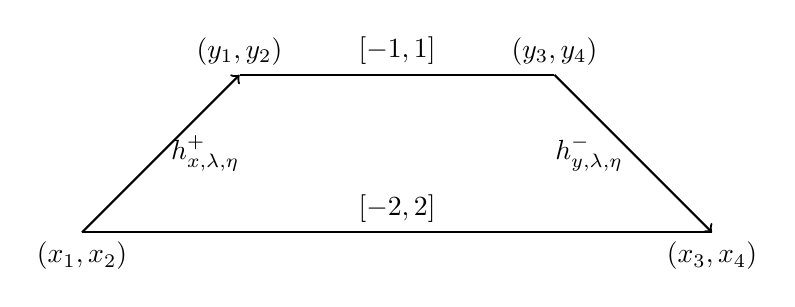
\begin{tikzpicture}[scale=2]
    % Define coordinates for the intervals
    \coordinate (A) at (-2, 0);
    \coordinate (B) at (2, 0);
    \coordinate (C) at (-1, 1);
    \coordinate (D) at (1, 1);

    % Draw the intervals
    \draw[thick] (A) -- (B) node[midway, above] {$[-2, 2]$};
    \draw[thick] (C) -- (D) node[midway, above] {$[-1, 1]$};

    % Draw the transformation arrows
    \draw[->, thick] (A) -- (C) node[midway, right] {$h_{x,\lambda,\eta}^+$};
    \draw[<-, thick] (B) -- (D) node[midway, left] {$h_{y,\lambda,\eta}^-$};

    % Label the points
    \node at (A) [below] {$(x_1, x_2)$};
    \node at (B) [below] {$(x_3, x_4)$};
    \node at (C) [above] {$(y_1, y_2)$};
    \node at (D) [above] {$(y_3, y_4)$};
\end{tikzpicture}

\end{document}